\section{Removing noisy MDT tubes}
\label{sec:noisytubes}

The MDTs are composed of hundreds of thousands of drift tubes. A small fraction of these tubes show noisy behavior such that they record hits at a much higher rate than expected from incident particles. They are therefore discarded from this analysis to avoid biasing the measurements, both in counting hit tubes and in deriving the active area of the MDTs.

Noisy tubes are identified by observing the tube-level occupancy in Run 284285. As shown in Figure~\ref{fig:noisytubes}, the long tail at high occupancy indicates that a few tubes fire 1-2 orders of magnitude more often than most. Judging the spectrum by eye, tubes are marked as noisy if they fired in more than 10\% of events in Run 284285.

\begin{figure}
  \begin{center}
    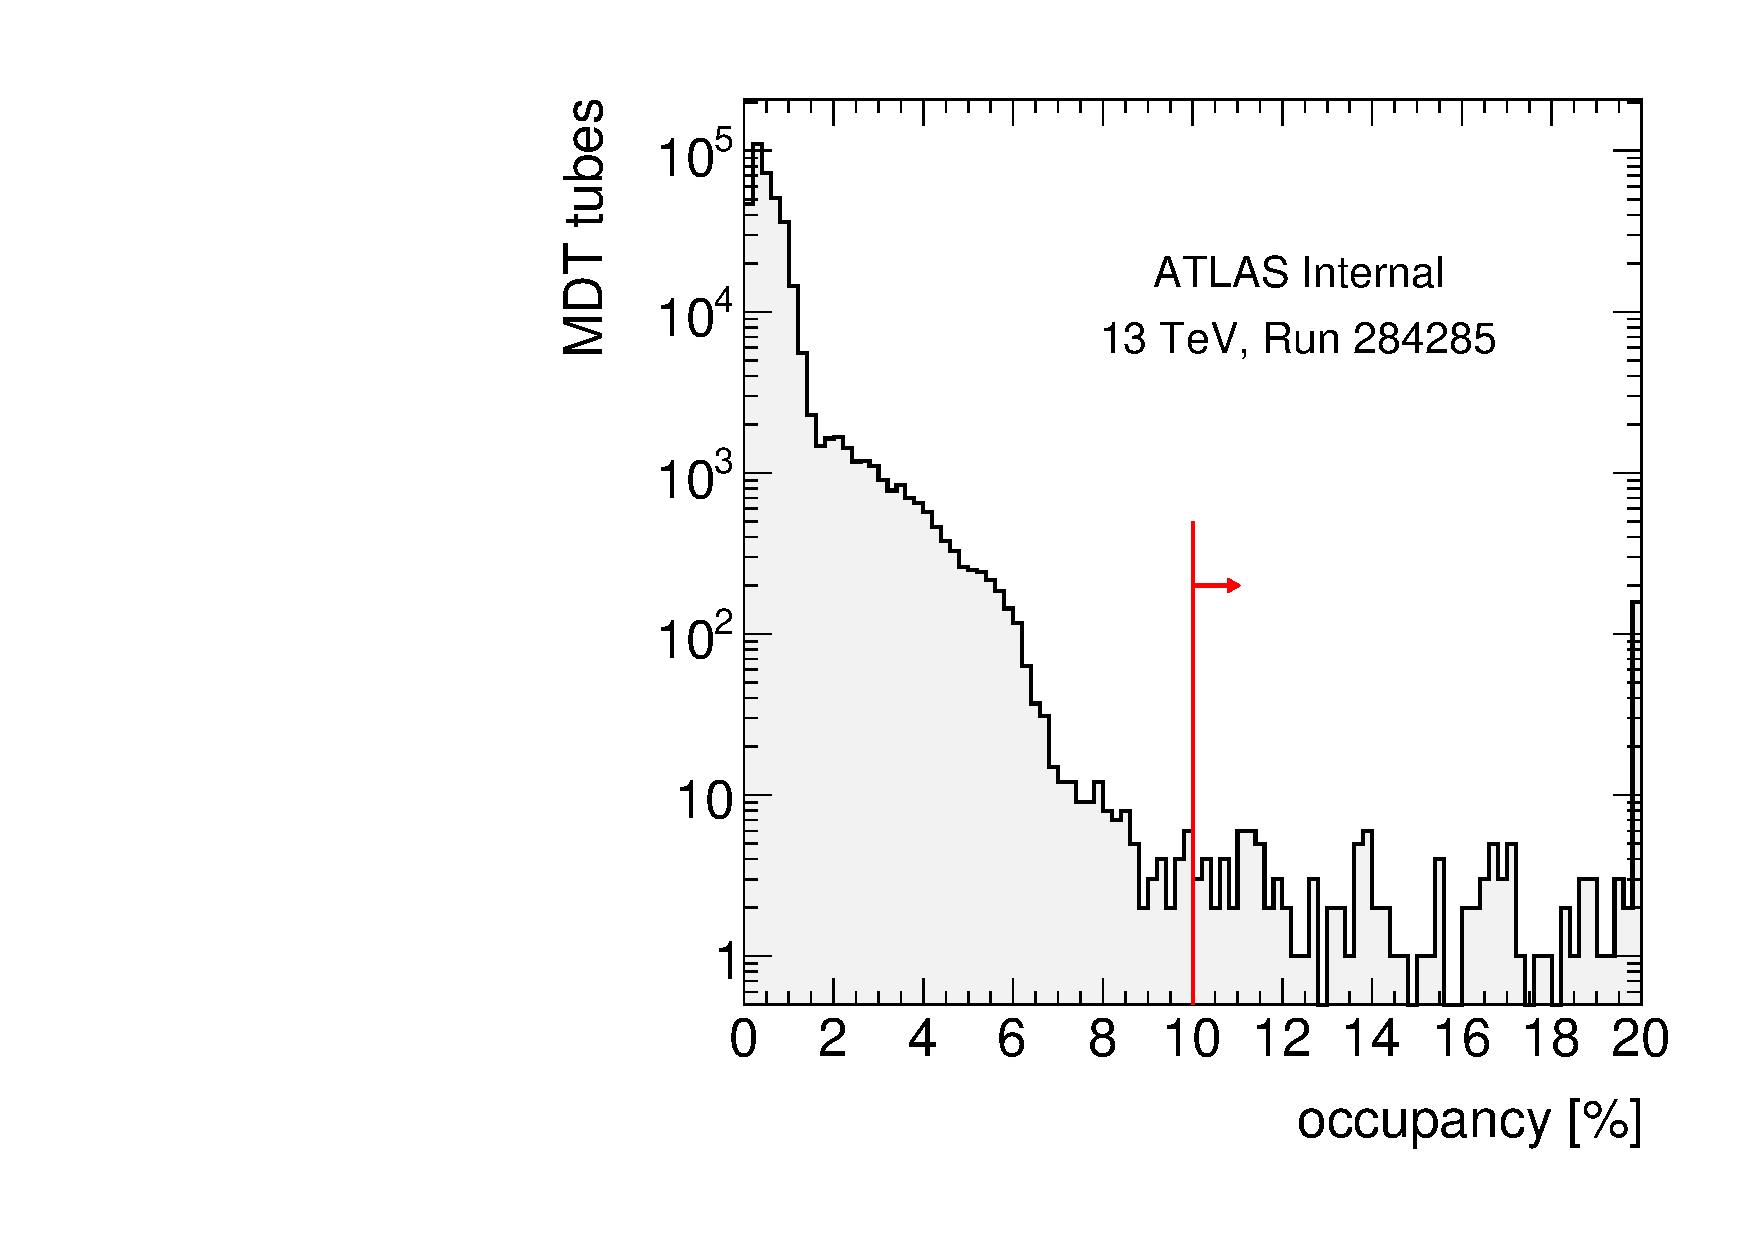
\includegraphics[width=0.45\textwidth]{./figures/occupancy_00284285.pdf}
    \caption{MDT tube occupancy in Run 284285. Most tubes fire in less than 2\% of events, but some fire at much larger rates. Tubes which fire in greater than 10\% of events in Run 284285 are considered noisy and discarded in this analysis.}
    \label{fig:noisytubes}
  \end{center}
\end{figure}


